\documentclass[12pt]{article}
\usepackage{parskip}
\usepackage{amsmath}
\usepackage{pdfpages}
\usepackage{listings}
\usepackage{color}
\usepackage[margin=.6in]{geometry}

\definecolor{dkgreen}{rgb}{0,0.6,0}
\definecolor{gray}{rgb}{0.5,0.5,0.5}
\definecolor{mauve}{rgb}{0.58,0,0.82}

\lstset{frame=tb,
  language=C++,
  aboveskip=3mm,
  belowskip=3mm,
  showstringspaces=false,
  columns=flexible,
  basicstyle={\small\ttfamily},
  numbers=none,
  numberstyle=\tiny\color{gray},
  keywordstyle=\color{blue},
  commentstyle=\color{dkgreen},
  stringstyle=\color{mauve},
  breaklines=true,
  breakatwhitespace=true,
  tabsize=3
}
\begin{document}
The first set of slides is a simple introduction with no real content. Memorize these vocabulary words.

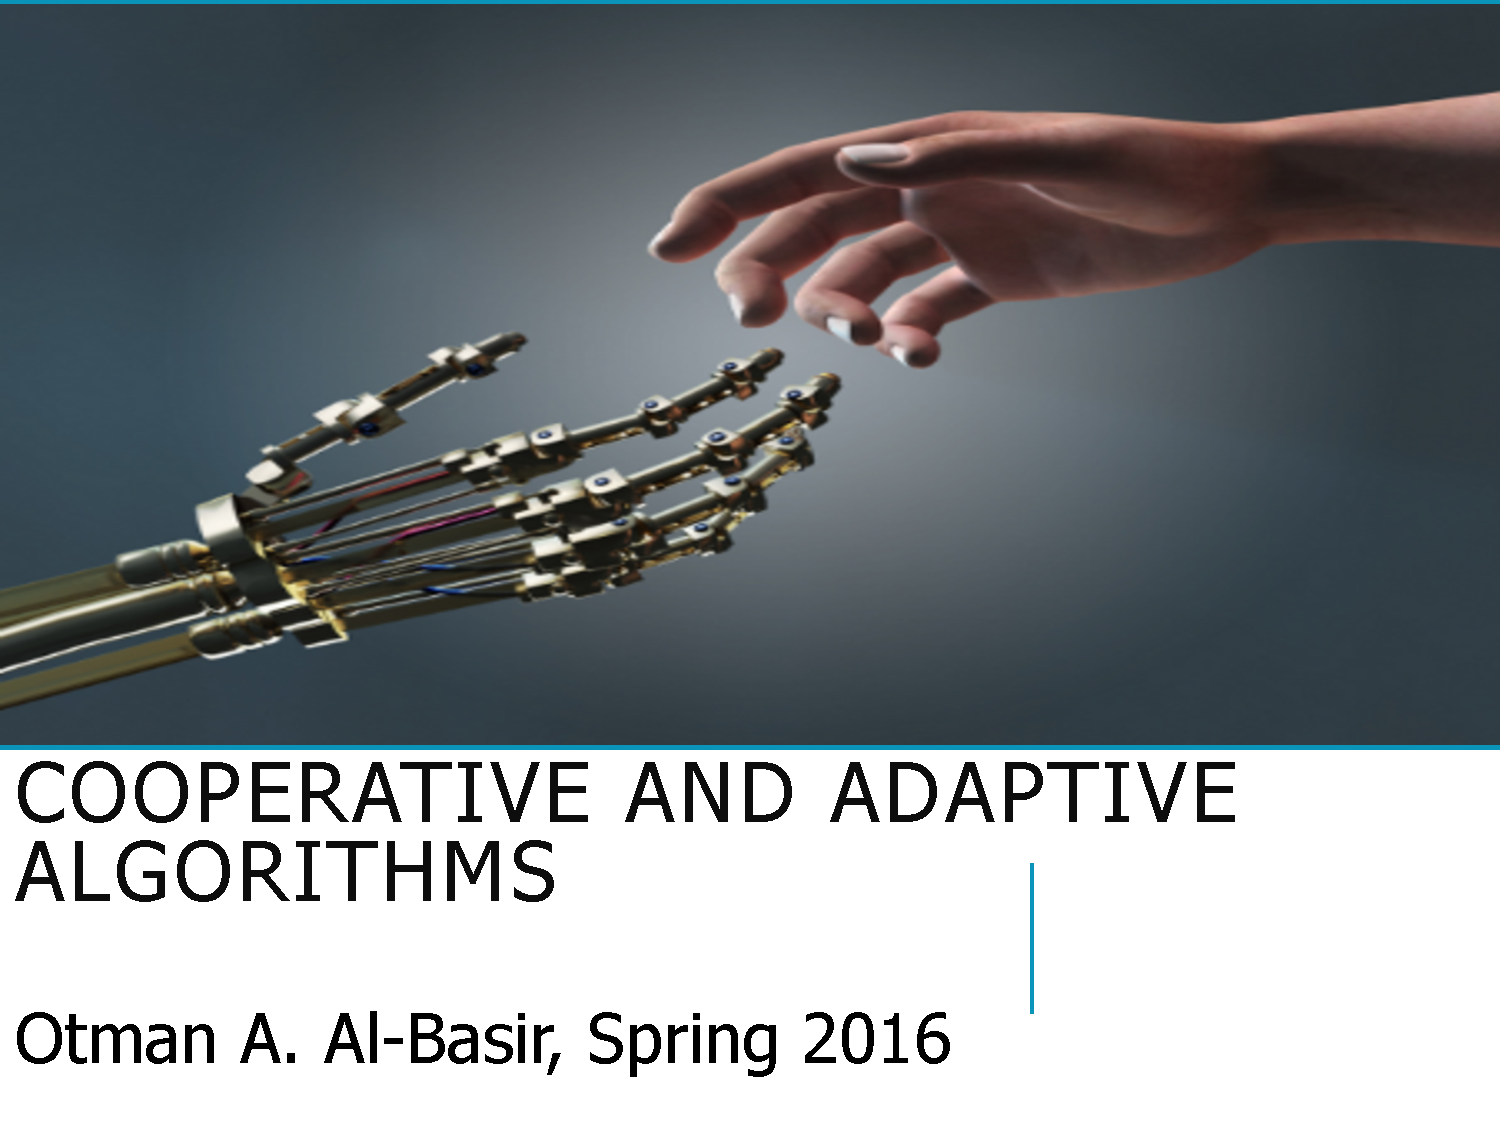
\includepdf[pages=1-41]{slides.pdf}
We want to find a solution with the least cost possible. So we need to have a thing to find and away to evaluate the cost of finding that thing.
\includepdf[pages=42]{slides.pdf}
We need to be able to represent our space in a way for computers to easily manage (usually making it binary). From there we get a goal, a solution, and
\end{document}